\documentclass{article}
% General document formatting
\usepackage[margin=0.7in]{geometry}
\usepackage[parfill]{parskip}
\usepackage[utf8]{inputenc}
\usepackage{hyperref} 
\usepackage{booktabs}
\usepackage{graphicx}
\usepackage{subfig}
\usepackage{caption}
\usepackage{fancyhdr}

% Related to math
\usepackage{amsmath,amssymb,amsfonts,amsthm}
\title{Design, Implementation and evaluation of different strategies for playing Pokémon battles \\ Proposal}
\author{Julian Schubert}

% Kopf- / Fußzeile
\makeatletter
\let\runauthor\@author
\let\runtitle\@title
\pagestyle{fancy}
\fancyhf{}
\rhead{Proposal}
\lhead{\runauthor}
\cfoot{\thepage}

\begin{document}
\maketitle

\section{Introduction}
Pokémon is a video game series created by the Pokémon Company.
The goal of the game is to not only catch Pokémon, but also to train them and use
them to battle other trainers. In the mainline games, the focus lies on the story
as well as exploring the world. The Pokémon genre has evolved quite a bit since
its early days, Figures \ref{fig:red0} and \ref{fig:red1} contain screenshots 
of the first Pokémon games, Pokémon Red and Pokémon Green.
\begin{figure}[ht]
    \centering
    \begin{minipage}{.5\textwidth}
      \centering
      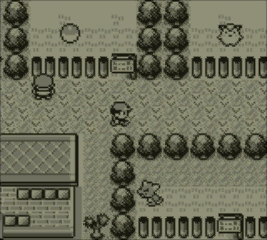
\includegraphics[width=.9\linewidth]{images/Red-0.jpg}
      \captionof{figure}{Exploring the map in Pokémon Red}
      \label{fig:red0}
    \end{minipage}%
    \begin{minipage}{.5\textwidth}
      \centering
      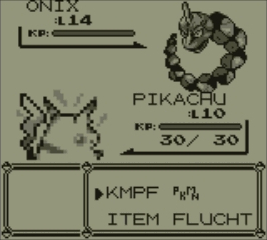
\includegraphics[width=.9\linewidth]{images/Red-1.jpg}
      \captionof{figure}{Fighting another trainer in Pokémon Red}
      \label{fig:red1}
    \end{minipage}
    \caption*{Image source: \href{https://www.nintendo.de/Spiele/Game-Boy/Pokemon-Rote-Edition-266109.html}{nintendo.de}}
\end{figure}
Figures \ref{fig:sword0} and \ref{fig:sword1} contain in game footage of the latest games in
the series, Pokémon Sword and Shield.
\begin{figure}
  \centering
  \begin{minipage}{.48\textwidth}
    \centering
    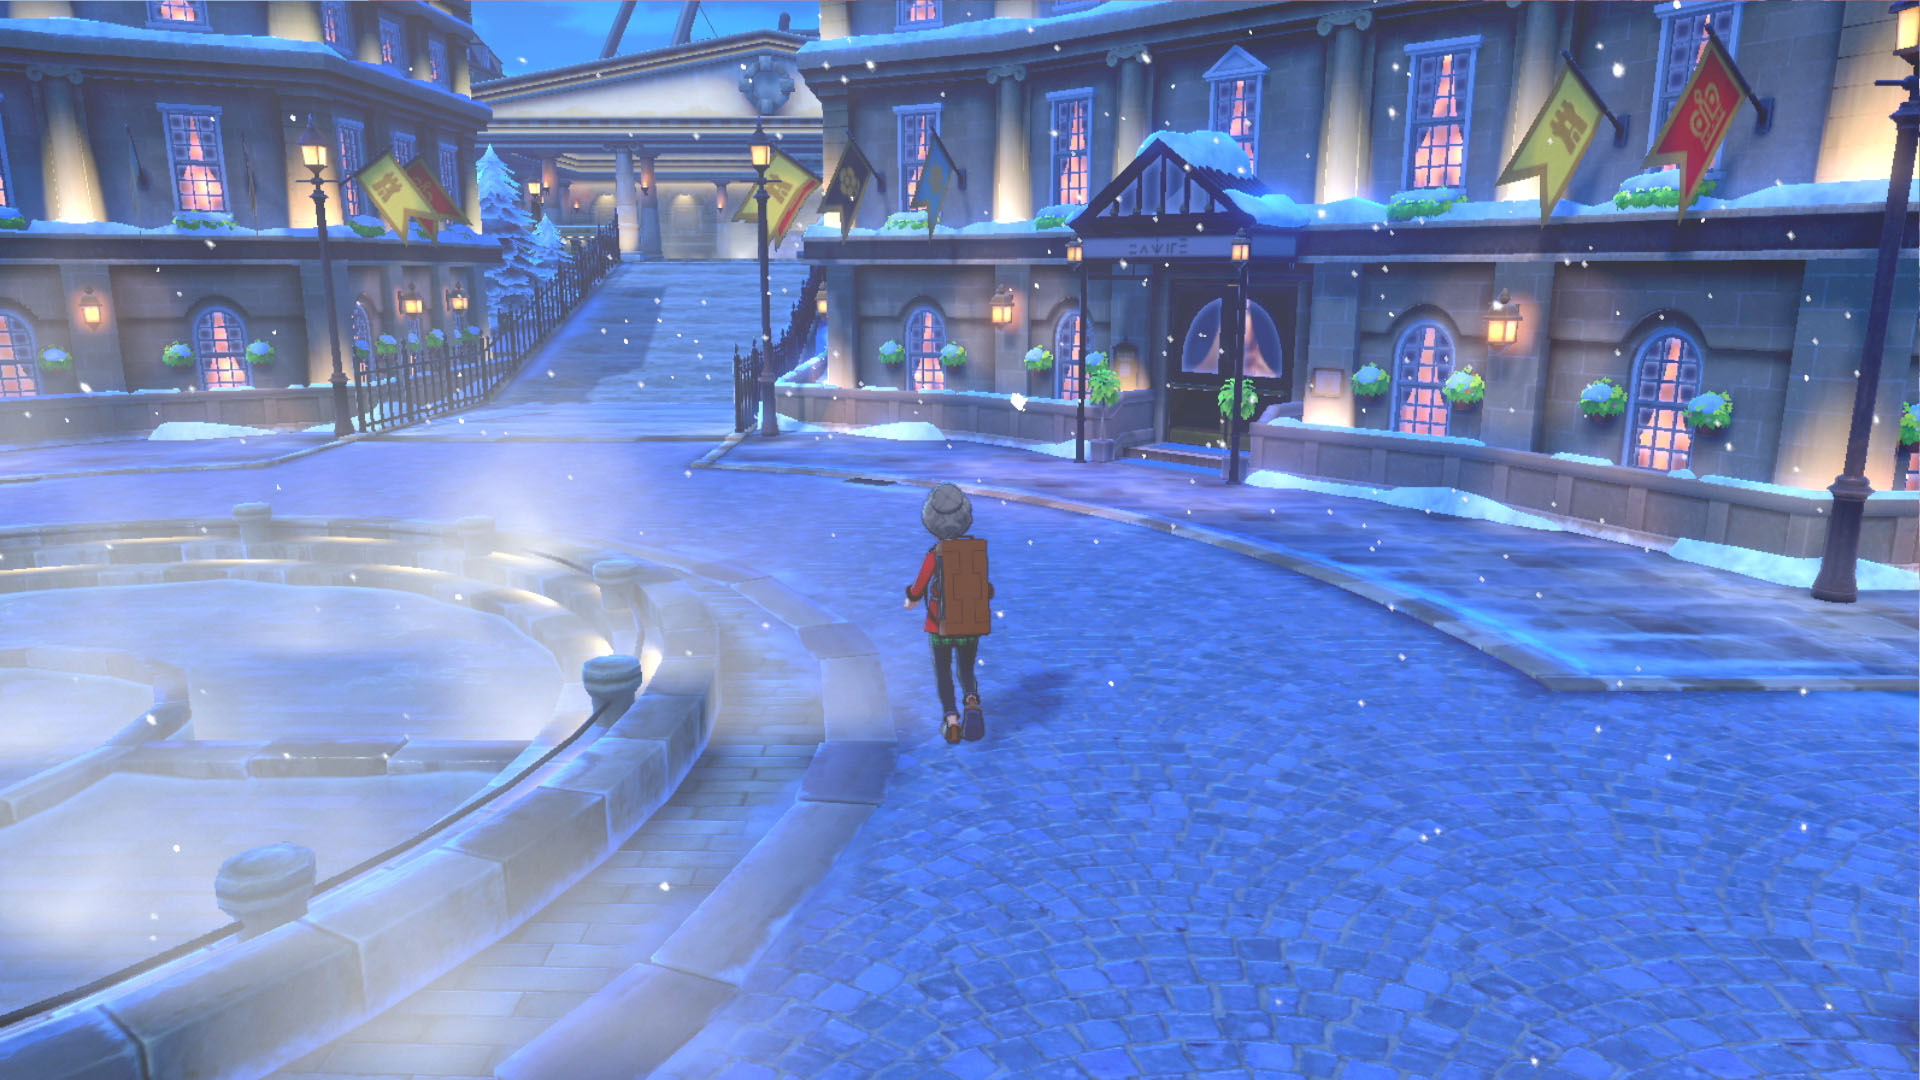
\includegraphics[width=.9\linewidth]{images/Sword-0.jpg}
    \captionof{figure}{Exploring the map in Pokémon Sword. \\ 
      Image source: \href{https://swordshield.pokemon.com/de-de/gameplay/pokemon-battle-stadium/}{pokemon.com}}
    \label{fig:sword0}
  \end{minipage}%
  \begin{minipage}{.48\textwidth}
    \centering
    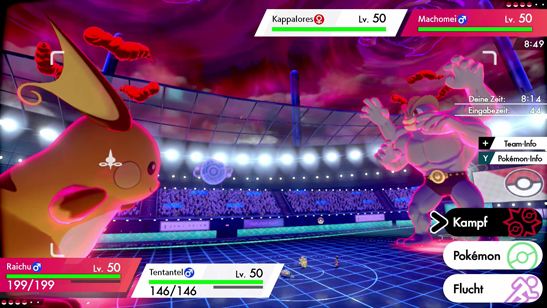
\includegraphics[width=.9\linewidth]{images/Sword-1.jpg}
    \captionof{figure}{Fighting another trainer in Pokémon Sword \\
      Image source: \href{https://www.nintendo.de/Spiele/Nintendo-Switch/Pokemon-Schwert-1522111.html}{nintendo.de}}
    \label{fig:sword1}
  \end{minipage}
\end{figure}
This thesis will focus exclusively on battling as there are detailed lists
of the locations of everything there is to explore within the games.

\section{Prerequisites}
Nintendo does not provide an API for the game, however, the fan project
\href{https://play.pokemonshowdown.com/}{Pokemon Showdown} is a
free online tool that can be used to battle online trainers. On top of that,
it provides the functionality to use their simulator offline in an CLI. The
entire source code for Pokémon Showdown can be found at 
\href{https://github.com/smogon/pokemon-showdown}{Github}.
Additionally, the python library \href{https://poke-env.readthedocs.io/en/latest/}{poke-env}
is used as it provides a convenient interface to Showdown. \\
The combination of both tools allows to easily perform deep reinforcement learning
on a local running instance of Showdown, and evaluating models against 
human players on the official Pokémon Showdown server. Figure \ref{fig:showdown-battle}
shows a battle between two human players on Pokémon Showdown. Lastly, the creators
of Pokémon Showdown provided me with over 8 Million replays of games played
by humans.

\section{Battling}
There are multiple popular battle formats in Pokémon as well as in Pokémon
Showdown. This research will focus exclusively on the most popular category
on Showdown: Random battles with Pokémon from all different games. \\
\textit{Note:} In the mainline games items also play a huge role in battle,
as they for example allow the revival of a fainted Pokémon. In competitive
play items are banned, only held items allowed. A held item can for example
allow a Pokémon to more often be able to attack first or trade in defensive
stats for offensive ones.

\subsection{Fundamentals}
At the start of the game, each player gets 6 different random Pokémon. A player
knows all 6 Pokémon he has with all their available moves, yet, he only knows
the active Pokémon of his opponent. Additionally, the player does not know what
moves the opposing Pokémon is able to use. Each Pokémon knows 4 different moves,
a move can either \textit{attack}, \textit{strengthen} himself or the own team,
or \textit{weaken} the enemy Pokémon or team by for example poisoning the enemy
Pokémon. \\ 
Pokémon battles are turn based. Each turn, both players either choose a move
for their active Pokémon, or switch to another Pokémon of the team. 

\subsection{Type advantages}
\begin{figure}[ht]
  \centering
  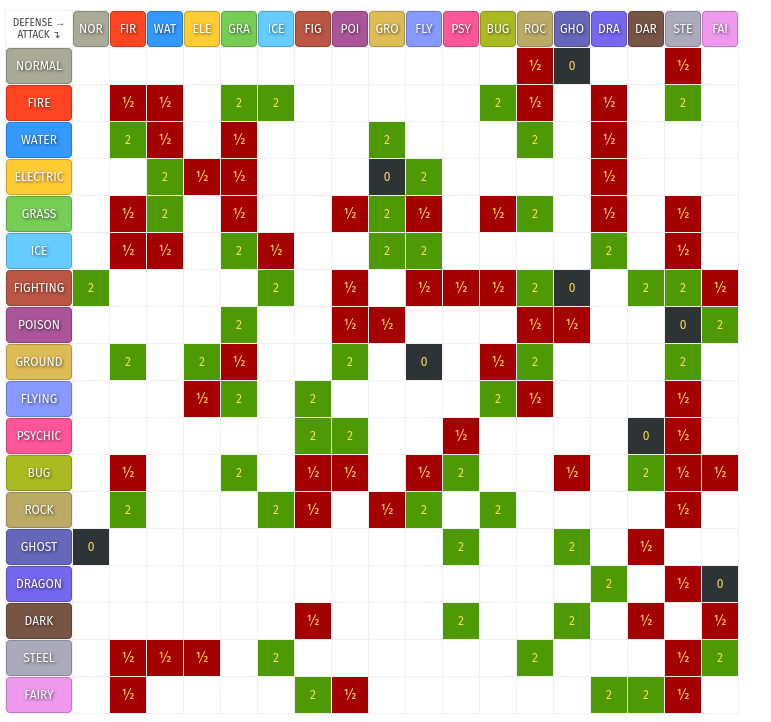
\includegraphics[width=.9\linewidth]{images/Types.png}
  \captionof{figure}{Type chart \\
    Image source: \href{https://pokemondb.net/type}{pokemondb.net}}
  \label{fig:type-chart}
\end{figure}
The game implements rock-paper-scissors-like system. Each Pokémon has one
or two types, each move has a type as well. A Pokémon has a \textit{type advantage}
against another Pokémon, if his moves deal extra damage against the opposing Pokémon.
Figure \ref{fig:type-chart} shows how every type interacts with every other type.
For example, a \textbf{Fire} deals normal damage against \textbf{Electric}, twice
as much damage against \textbf{Bug} and only half amount of damage against
\textbf{Rock}. \\
\textit{Note:} These damage modifiers are multiplied with each other, so if a 
fire move were to hit a Pokémon with type electric and bug, the move would
deal the usual amount of damage.

\subsection{Showdown battle interface}
Figure \ref{fig:showdown-battle} is taken from an ongoing battle on Pokémon
Showdown. The red marking shows the remaining hit points (hp) of player one's
active Pokémon. As the bar is completely full, the Pokémon still has 
not taken any damage. Once a Pokémon has no health remaining, it faints,
and the player has to switch to another Pokémon. 
The enemy Pokémon
only has 33\% of its health remaining. As highlighted by the green 
marking, the enemy Pokémon is called "Kommo-o", is male and has
level 80. In the blue marked area, the status effects are displayed. For
example, the attack-stat of "Kommo-o" is raised by 50\%. Framed
yellow is the team of the opposing player. Both grayed out
Pokémon are fainted and therefore can't be sent into battle,
the fully colored Pokémon are still alive and the ball in
the bottom right corner indicates one unknown Pokémon the 
player hasn't sent out yet. \\
Below that, the four moves the Mewtwo can pick from are displayed.
In this case, these moves are \textbf{Fire Blast}, \textbf{Recover},
\textbf{Psystrike} and \textbf{Nasty Plot}.

\begin{figure}[ht]
  \centering
  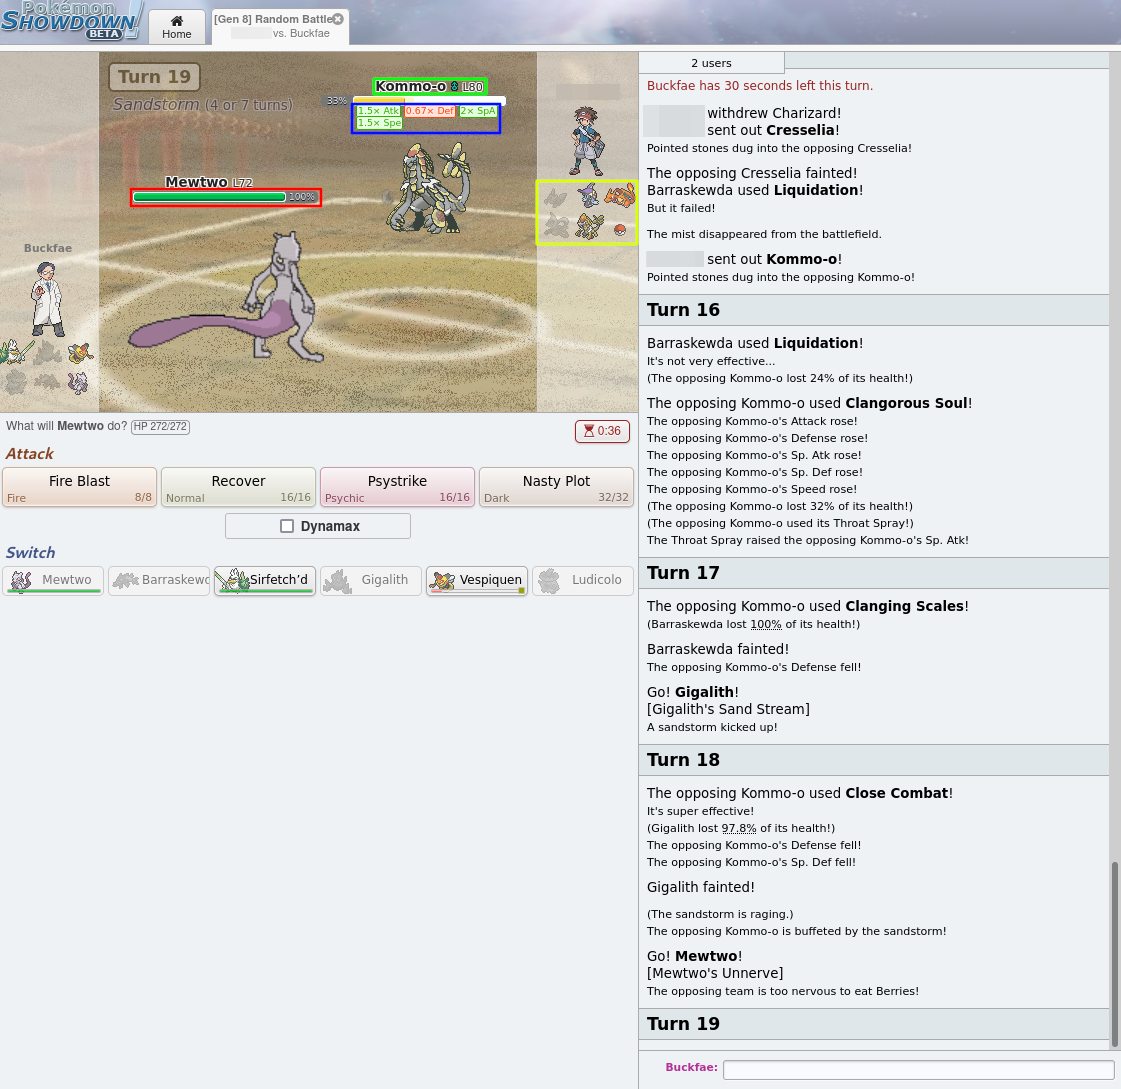
\includegraphics[width=.9\linewidth]{images/Showdown.png}
  \captionof{figure}{Screenshot of me battling a random opponent}
  \label{fig:showdown-battle}
\end{figure}

\subsection{Advanced battling strategies}
In section \ref{sec:rulebased} a simple rule-based approach is introduced that 
always picks the move that deals the most amount of damage. However, picking 
an optimal move is a lot more complex than this. Pokémon battles are not just
strict one on one battles where the player with the most damage dealing Pokémon
always wins. In competitive play, a wide variety of non- or low-damaging moves
is used. Dragon Dance for example, does not deal any damage to the opponent, 
but increases the damage the Pokémon deals in the next turns. \\
Additionally, each Pokémon can play one or more different roles where the 
play styles, again, counter each other in a rock-paper-scissors-like fashion. 
Identifying in a random team what play style to pick for which Pokémon is
essential to winning battles. This decision is also based on the play styles
the opponent chooses. \\
Lastly, predicting enemy decisions is a key component of competitive play. For 
example, if the Pokémon of player one has a type advantage against the Pokémon 
of player two, the opposing player may switch to another Pokémon. As a possible
counter-play, the first player could pick a move that will deal less damage
against the current opposing Pokémon but is also good against the Pokémon
he assumes the enemy to switch to. \\
These elements turn competitive Pokémon in a game where traditional strategy
and probability management are combined with information management.

\section{Execution}
This thesis will investigate multiple possible approaches to optimize battling.
The first approach will be rule-based. Different complexity levels will be
tested against each other. Knowledge extracted from replays will be used to design the 
rules. \\
In addition, a reinforcement learning algorithm will be tested. The possibility 
to pretrain the network using either rules or replay data will be investigated as well.

\section{Evaluation}

The poke-env library provides not only a random player, but also a max damage player
that always chooses the move with the highest base damage. A simple RL
approach is given as well. These three agents will be used as baseline. \\
Pokémon Showdown also has an elo rating system similar to chess. The authors of 
Showdown allow bots to compete in ranked matches, so the approaches
developed in this thesis will also be evaluated by playing ranked games 
against actual humans.

\section{Example rule-based approach}
\label{sec:rulebased}
During testing of the technical feasibility of this approach, I developed a 
simple rule-based approach.

\subsection{Damage Calculation}
The expected damage a move will deal to an opposing Pokémon is calculated as follows:
\begin{equation*}
    \text{Expected Damage} = \text{Move Base Damage} \times \text{Move Type Modifier} 
        \times \text{Stab Modifier}
        \times \text{Move Accuracy}
\end{equation*}
\textbf{Stab Modifier}: If the type of the move is equal to one of the possibly two types
of the Pokémon, the move will deal 1.5 times more damage. 

\subsection{Rules for playing}
Deciding on the next move is purely based on the expected damage in the current turn.
If a Pokémon faints, the next Pokémon to switch in is picked based on the expected
damage it can deal to the opposing Pokémon.

\subsection{Evaluation}
This approach was evaluated against a random player and a player that always chooses
the move with the highest base damage. In 500 games, this approach won 484 out of 500
games against the random player and 419 / 500 games against the player that always chooses
the move with the highest base damage. \\
After training the example DQN-Agent proposed in the
\href{https://poke-env.readthedocs.io/en/latest/rl_with_open_ai_gym_wrapper.html}{poke-env documentation}
for 1 Million steps, this rule-based approach was able to win 666 out of 1,000 games. In ranked matches
against actual players, this rule-based approach was only able to win about one in three games, resulting
in the player getting stuck in the lowest elo group\footnote{In Pokémon Showdown, you can't have less
than 1,000 elo}.
\section{Time Management}
Following table shows the general timeline for this thesis. 
\begin{table}[ht]
    \centering
    \begin{tabular}{|l|c|c|c|c|c|c|c|c|c|c|}
    \hline
     & \multicolumn{9}{c}{Time in weeks}  & \\ \hline
     & \textbf{1} & \textbf{2} & \textbf{3} & \textbf{4} & \textbf{5} & \textbf{6} & \textbf{7} & \textbf{8} & \textbf{9} & \textbf{10} \\ \hline
    Mechanics of the game                       & x &   &   &   &   &   &   &   &   &   \\ \hline
    Extracting Data from replays                &   & x &   &   &   &   &   &   &   &   \\ \hline
    Rule-based approach: Implementation          &   &   & x & x &   &   &   &   &   &   \\ \hline
    Buffer                                      &   &   &   &   & x &   &   &   &   &   \\ \hline
    Reinforcement learning: Research            &   &   &   &   &   & x &   &   &   &   \\ \hline
    Reinforcement learning: Implementation      &   &   &   &   &   &   & x & x &   &   \\ \hline
    Writing                                     & x & x & x & x & x & x & x & x & x & x \\ \hline
    \end{tabular}
    \caption{Time Management in weeks}
\end{table}
\end{document}